\section[Využití jaderně-fyzikálních metod v materiálovém výzkumu]{Využití jaderně-fyzikálních metod v materiálovém výzkumu: Mössbauerova spektrometrie, elektron-pozitronová anihilační spektroskopie, neutronová aktivační analýza}

\subsection{Mossbauerova spektrometrie}

Byla objevena německým fyzikem Rudolfem Mossbauerem v roce 1958. Je založeno na rezonanční fluorescenci $\gamma$ záření

Obvykle používané prvky: $^{57}$Fe, $^{119}$Sn, $^{121}$Sb, $^{129}$I.

Široká škála aplikací při studiu chemických vazeb, anorganické chemii pevných látek, atd. Hlavní množství článků a studií je ale zaměřeno na železo.

Jedná se o metodu izotopicky citlivou (bezodrazová jaderná rezonanční absorpce/fluorescence gama záření).

\subsubsection{Princip}

Mossbauerův jev = bezodrazová jaderná rezonanční absorpce gamma záření

\begin{itemize}
    \item Založeno na emisi a absorpci $\gamma$ záření emitovaného jádrem bez zpětného rázu.
    \item Atomy ve zdroji emitující $\gamma$ záření musí být stejné, jako v atomy ve vzorku.
    \item Vlastně je to tak, že jádra ve vzorku jsou excitovaná gammou, která je emitovaná při stejné deexcitaci ve zdroji.
    \item Zde zdroje fotnů jsou generovány fotony o dané energii a pokud je tato energie veeeelmi přesná jako je energie mezi vzbuzeným a základním stavem atomu či jádra ve zkoumaném materiálu, tak dojde k tzv. rezonanční absorpci.
    \item Poté dochází opět k přechodu zkoumaného jádra do základního stavu emisí fotonu o té samé energii, co to původně vyvolala
    \item Celé co chceme je dosáhnout překrycu emisní a absoprpční čáry, což je velmi složité neboť je šířka píku (energie) velmi malá a komplikuje to celé jev tzv. zpětného rázu.
\end{itemize}

\subsubsection{Zpětný ráz}
\begin{itemize}

\item Při emisi vysokoenergetické částice z jádra funguje zpětný odraz, část hybnosti je předaná emitujícímu jádru (analogicky u zbraně -- taky mě to hodí trochu dozadu).
\item Energie gamma záření má proto o trošku nižší energii než je energie rezonance, a to o energii tohoto zpětného rázu.
\item Pro energii zpětného rázu platí: $E_{R} = \dfrac{E_{\gamma}}{2 M c^2}$, kde $M$ je hmotnost emitujícího jádra a $E_{\gamma}$ je energie emitovaného fotonu.
\item S narůstající hmotností $M$ klesá energie zpětného odrazu, a proto platí, že jeli energie emitovaného gama záření malá oproti hmotnosti jádra, jež jej emituje, pak se energie zpětného rázu pohltí a s jádrem to nehne. V opačném případě je třeba tuto energii nějak zohlednit a ideálně ji kompenzovat.
\item V případě nevázaného jádra je posun energie značný a není možné Mossbauerův jev pozorovat. Neboli nedojde k překryvu emisní a absorpční čáry.

Příkladem je známé železo Fe-57 u něhož je šířka čáry 4,6 neV a energie zpětného rázu je 2meV. To znamená, že emitované gama o velikosti 14.4 keV, které na něj letí s cílem ho excitovat, tak mi je k ničemu, protože energie fotonu je nižší o ty 2 meV a tudíž nedosáhnu překryvu emisní a absorpční čáry, která je ultra tenounká. Nutno dále zmínit, že o energii zpětného rázu se mi navíc posouvá nejen emisní čára, ale i absorpční čára, neboť to má vliv i na jádro, jež energii přijíma. Souhrně řečeno: U volného jádra (plynné či kapalné médium) dochází při emisi k zpětnému rázu, o který se sníží energie emitovaného fotonu a pak nevystačuje energie na excitaci cílového jádra.

\item Zvýšení hmotnosti jádra, aby byla energie zpětného rázu pohlcena/kompenzována lze dosáhnout uvázáním jádra do krystalické mřížky $\rightarrow$ zpětný ráz je daleko menší, do hmotnosti se taky připočítávají okolní vázané atomy, neboli mřížka tlumí odraz.
\end{itemize}


\textbf{Jak to funguje:}

\begin{itemize}
    \item Mám zdroj, který emituje přesně energii, kterou chci pro excitaci atomu/jádra v mém vzorku (pro tyto účely uvažujme Fe-57).
    \item Ve vzorku mám atomy/jádra Fe-57, které toto záření absorbují, jsou excitována a poté při deexcitaci emitují gama záření o té samé energii, která je excitovala z mého zdroje (jak bylo řečeno výše, tak zdrojem je to samé jádro, které chci ve vzorku excitovat. Toto jádro, které já beru jako zdroj tak excituju nějakým externím RN zdrojem například).
    \item Emitované záření ze vzorku je pak emitované do celého prostorového úhlu.
\end{itemize}

\begin{figure}[H]
    \centering
    \includegraphics[width=\linewidth]{img/Mossbauer excitace jádra.png}
    \caption{Mossbauer excitace jádra}
\end{figure}

\subsubsection{Pravděpodobnost jevu}

Celá pravděpodobnost, že nastane tento jev je popsána skrze účinný průřez rezonanční absorpce závisející na spinu základního a excitovaného jádra, vlnové délce fotonů a na šířce čáry.

%- účinný průřez rezonanční absorpce 

$$\sigma_0 = \dfrac{\lambda^2}{2\pi} \cdot \dfrac{2I_e + 1}{2I_g +1} \cdot \dfrac{1}{1+\alpha},$$

kde $I_{g,e}$ jsou jaderné spiny základního a rezonančního stavu, $\alpha$ koeficient vnitřní koverze a $\lambda$ vlnová délka fotonu.
 
 % - pak je tam vzorec pro výpočet počtu přechod mezi $E-E_0$ a $E-E_0 + dE$, poocí f-faktoru
 
Dále hraje roli, tzv f-faktor, který popisuje pravděpodobnost bezfononového procesu. Tento faktor závisí na silách v mřížce a tedy čím více mřížka vibruje, tím více bude f-faktor klesat. Pravděpodobnost Mossbauerova jevu tedy roste se snižující se energií gama fotonu (menší zpětný odraz), roste se snižující se teplotou (menší tepelný pohyb) a roste se zvyšující se Debeyeovou teplotou (popisuje míru síly vazeb mezi jádrem a okolní mřížkou, resp. obecně míru síly vazeb).
 
 %- pro ideální experiment musí platit, že výchylka atomů je malá v  porovnání s vlnovou délkou gamma záření, teplota je menší než Debeyova teplota, energie přechodu není příliš vysoká (< 150 keV) a energie zpětného rázu je malá
 
Mossbauerovou spektormetrii lze měřit pouze krystalické a amorfně tuhé látky, zamrznuté roztoky (enmohu kapaliny a plyny).

\subsubsection{Uspořádání experimentu}

Základní součástí experimentu je zdroj záření, zkoumaný vzorek a detektor. Ne každý izotop je však vhodný pro zkoumání a měření touto metodou (již řečeno).

Aparatura se skládá z:

\begin{itemize}
    \item Zdroj/zářič: Nejvíce využívaný je izotop Fe-57, dále je Sn-119 či Au nebo Eu. Hlavní je ale to železo.
        \begin{itemize}
            \item Omezení zkoumání vzorků na ty, které obsahují např. právě to Fe-57
            \item Energie fotonu musí být v určitém rozmezí energií, a proto to nefunguje pro všechny jádra (nad 180 keV je energie zpětného rázu moc velká a pod 5 keV se neprojevuje rezonanční absorpce).
            \item Potřebuji zdroj fotonů s velmi přesnou energií aby to fungovalo
            \item Požadavky na zdroj jsou tedy: Dostupnost, trvanlivost, šířka čáry
        \end{itemize}
    \item Absorbátor/zkoumaný vzorek: Pokud je vzorek moc tlustý pak dojde k úplné absorpci a nebudu mít žádný signál. Příliš tenký vzorek je ale také špatně, avšak existuje vztah pro výpočet efektivní tloušťky (pro železo je to 1-5 mg/cm2 Fe atomů).
    \item Detektor: V zásadě lze využít širokou škálu detektorů
        \begin{itemize}
            \item Scintilační NaI(Tl) -- nejvíce využívaný scintilák, pak existuje ještě na bázi Ytria, ale ten má na hovno energietické rozlišení a účinnost, ale má rychlou odezvu a je dobrý pro vysoké četnosti. Obecně jsou scintiláky dobré, jelikož jsou rychlé.
            \item Proporcionální (plynem plněný) -- lepší energetická rozlišovací schopnost (je to pravda?).
            \item Polovodičový -- na bázi Si či Ge, avšak pro tuto metodu je to možná až moc overkill a zbytečně drahé.
        \end{itemize}

    \item Pojezd zdroje -- Jelikož je překryv energií hodně malý, tak mohu jemnou modulací energie pomocí Dopplerovské modulace doladit, aby došlo k překryvu absorpčního a emisního píku. V praxi to provedu tak, že zdroj umístím na nějakou membránu a pohybuji s ním tam a zpět (kmitám) - lze si představit jako membrána u reproduktoru.
\end{itemize}

\textbf{Rozdělujeme 3 uspořádání při experimentu:}

Měřenní může v obecnosti trvat hodiny až dny nebo týdny, přičemž podmínky testu jsou statické. Mimo jiné mohu na zkoumaný materiál aplikovat nějaké vnější vlivy = magnetické pole, změna teploty apod.

\begin{itemize}
    \item Transmisní = Zdroj -- vzorek -- detektor. Měřím co je za vzorkem. Měřím tzv. emisní spektrum, protože měřím, to co mi ze vzorku vylétává

    \item Konverzní = Měřím jednak emitované gama záření, ale i RTG či konverzní elektrony, augerovy elektrony, čímž dostávám informace z různé hloubky, ovšem celkově je to stále jen desítky mikrometrů.

    \item Odrazová = Detektor je mimo osu primárního svazku a tím mám geometrii na odraz
\end{itemize}


\begin{figure}[H]
    \centering
    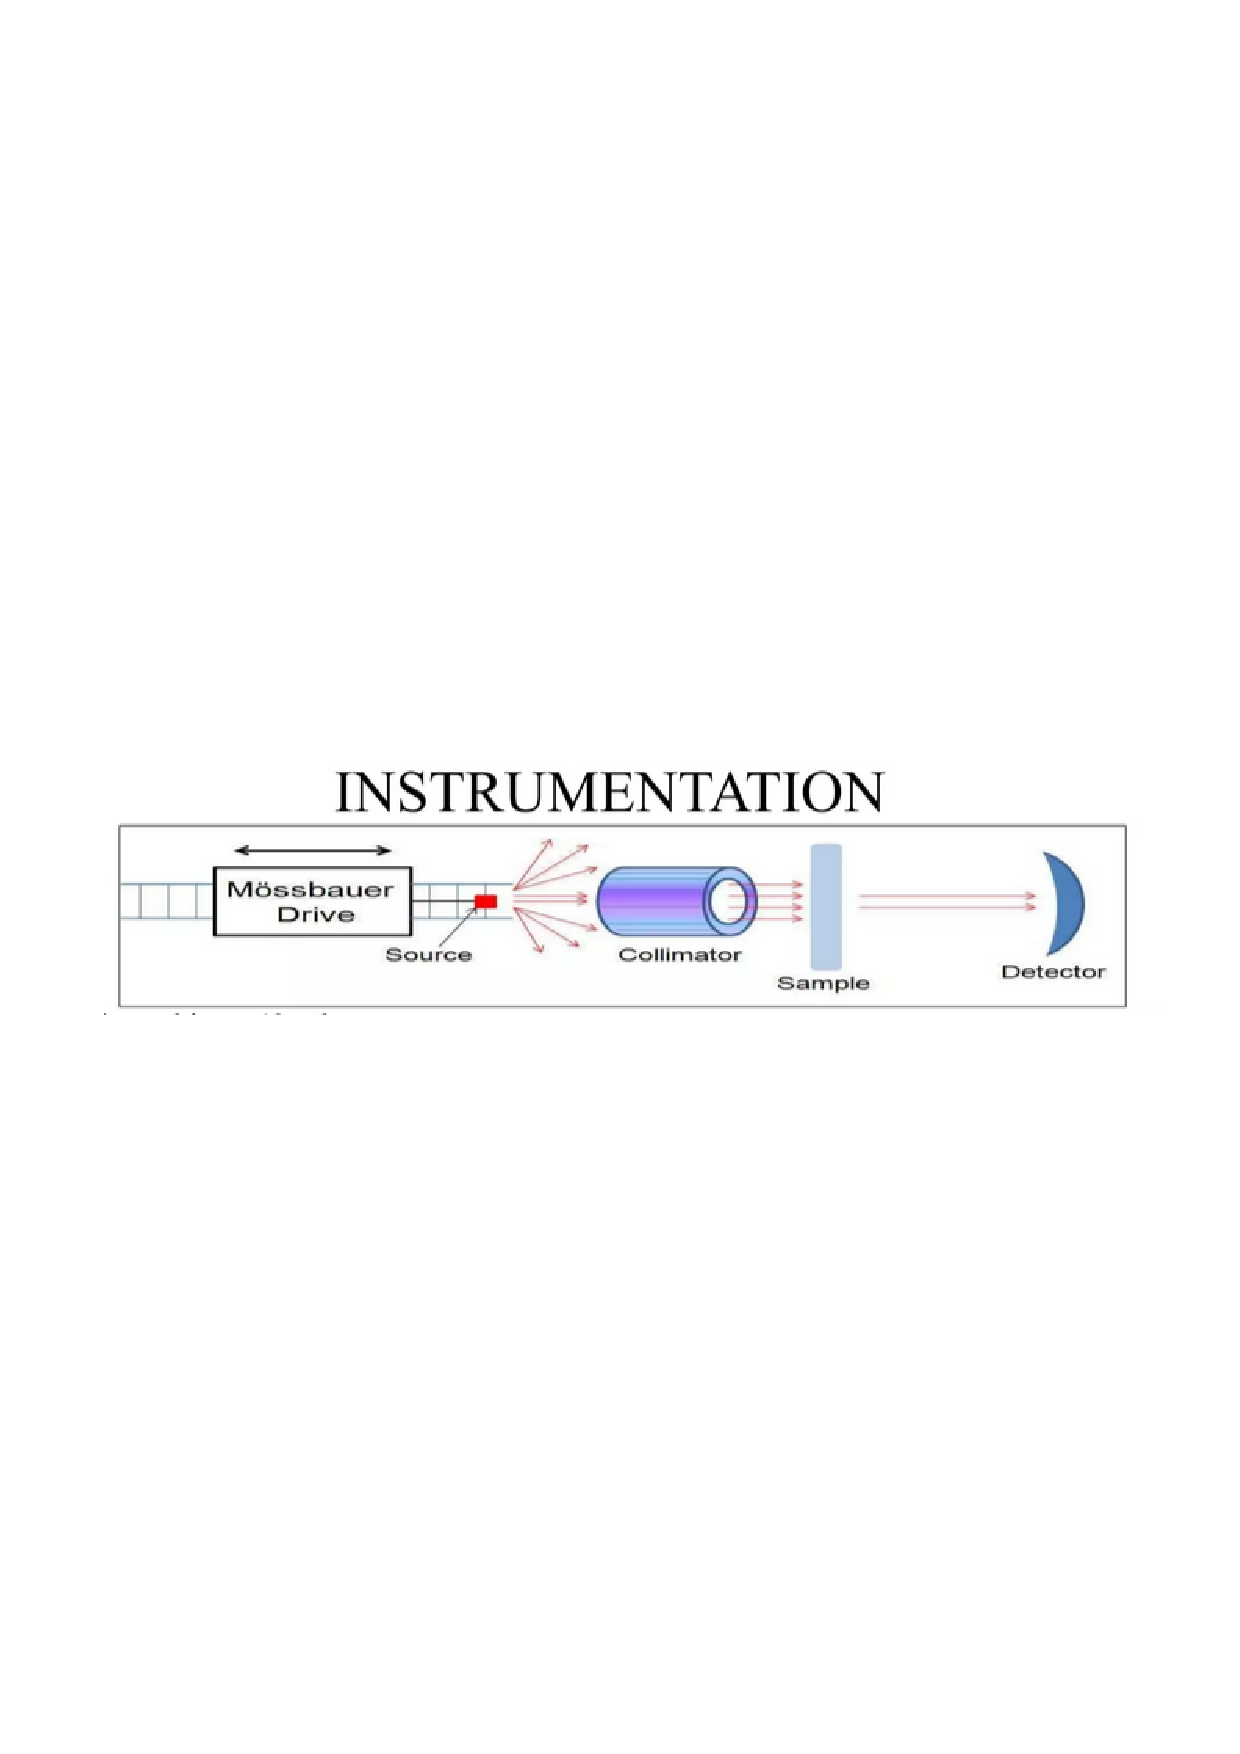
\includegraphics[width=0.8\linewidth, trim={1.5cm 11cm 1.5cm 11cm}, clip]{img/mossbauer_instrumentation.pdf}
    \caption{Experimentální uspořádání transmisní Mossbauerovy spektrometrie}
    \label{fig:2_6_mossbauer_zapojeni}
\end{figure}

%- můžu mít transmisní geometrii, odrazovou geometrii, můžu měřit konverzní elektrony
%- CEMS (Conversion Electrons Mossbauer Spectroscopy), TMS (Transmission Mossbauer Spectrometr), CXMS (Conversion X-ray Mossbauer Spectroscopy)
%- vzorek nesmí být ani moc tlustý, ani moc tenký - definuji efektivní tloušťku
%- jako detektory se využívají scintilárky, proporcionální detektory, polovodičové detektory nebo Si-PIN detektory
%- scintilační detektory NaI(Tl), YAP(Ce) 
%- proporcionální dteektory mají lepší rozlišení v porovnání se scintilákama
%

\subsubsection{Využití}

\begin{itemize}
    \item Mossbauerovské jádro mi funguje v mém materiálu jako sonda a říká mi informace o jeho okolí = lokální mikrostruktura
    \item Sledování hyperjmených interakcí Mossbauerovského jádra s jeho okolím = jedná se o interakce, které nějaký způsobem ovlivňují excitační stavy - Energetické stavy budou ovlivňovány svým okolím
    \item Mohu zkoumat vliv např. externího magnetického pole na posun či rozštěpení excitovaného či základního stavu (excitovaný/základní stav mají nějakou hladinu a buď může dojít vlivem externích jevů k jejich posuvu a nebo rozštěpení na více hladit)
    \item Informace o charakteru vazeb
    \item Informace o spinu
    \item Informace o oxidačním stavu
    \item Kvalitativní (identifikace sloučenin) i kvantitativní (poměrové zastoupení) např. fáze železa a jejich poměrové zastoupení i uspořádání. Interakce konkrétního nuklidu se svým okolím. 
    \item Využívá se především v materiálovém výzkumu a dále geologie, farmaceutický průmysl, biologie/medicín. Spíš ale prostě ten materiálový výzkum a je to.
\end{itemize}

\subsubsection{Hyperjemné interakce}

Jedná se o interakce, které nějaký způsobem ovlivňují excitační stavy, a to jak posunem nebo štěpením na více hladin. Bavíme se o:

\begin{itemize}
   \item elektrické monopólové interakci -- izomerický posun
   \item elektrická kvadrupólová -- kvadrupólové štěpení
   \item magnetická dipólová -- magnetické hyperjemné štěpení
\end{itemize}

\begin{figure}[H]
   \centering
   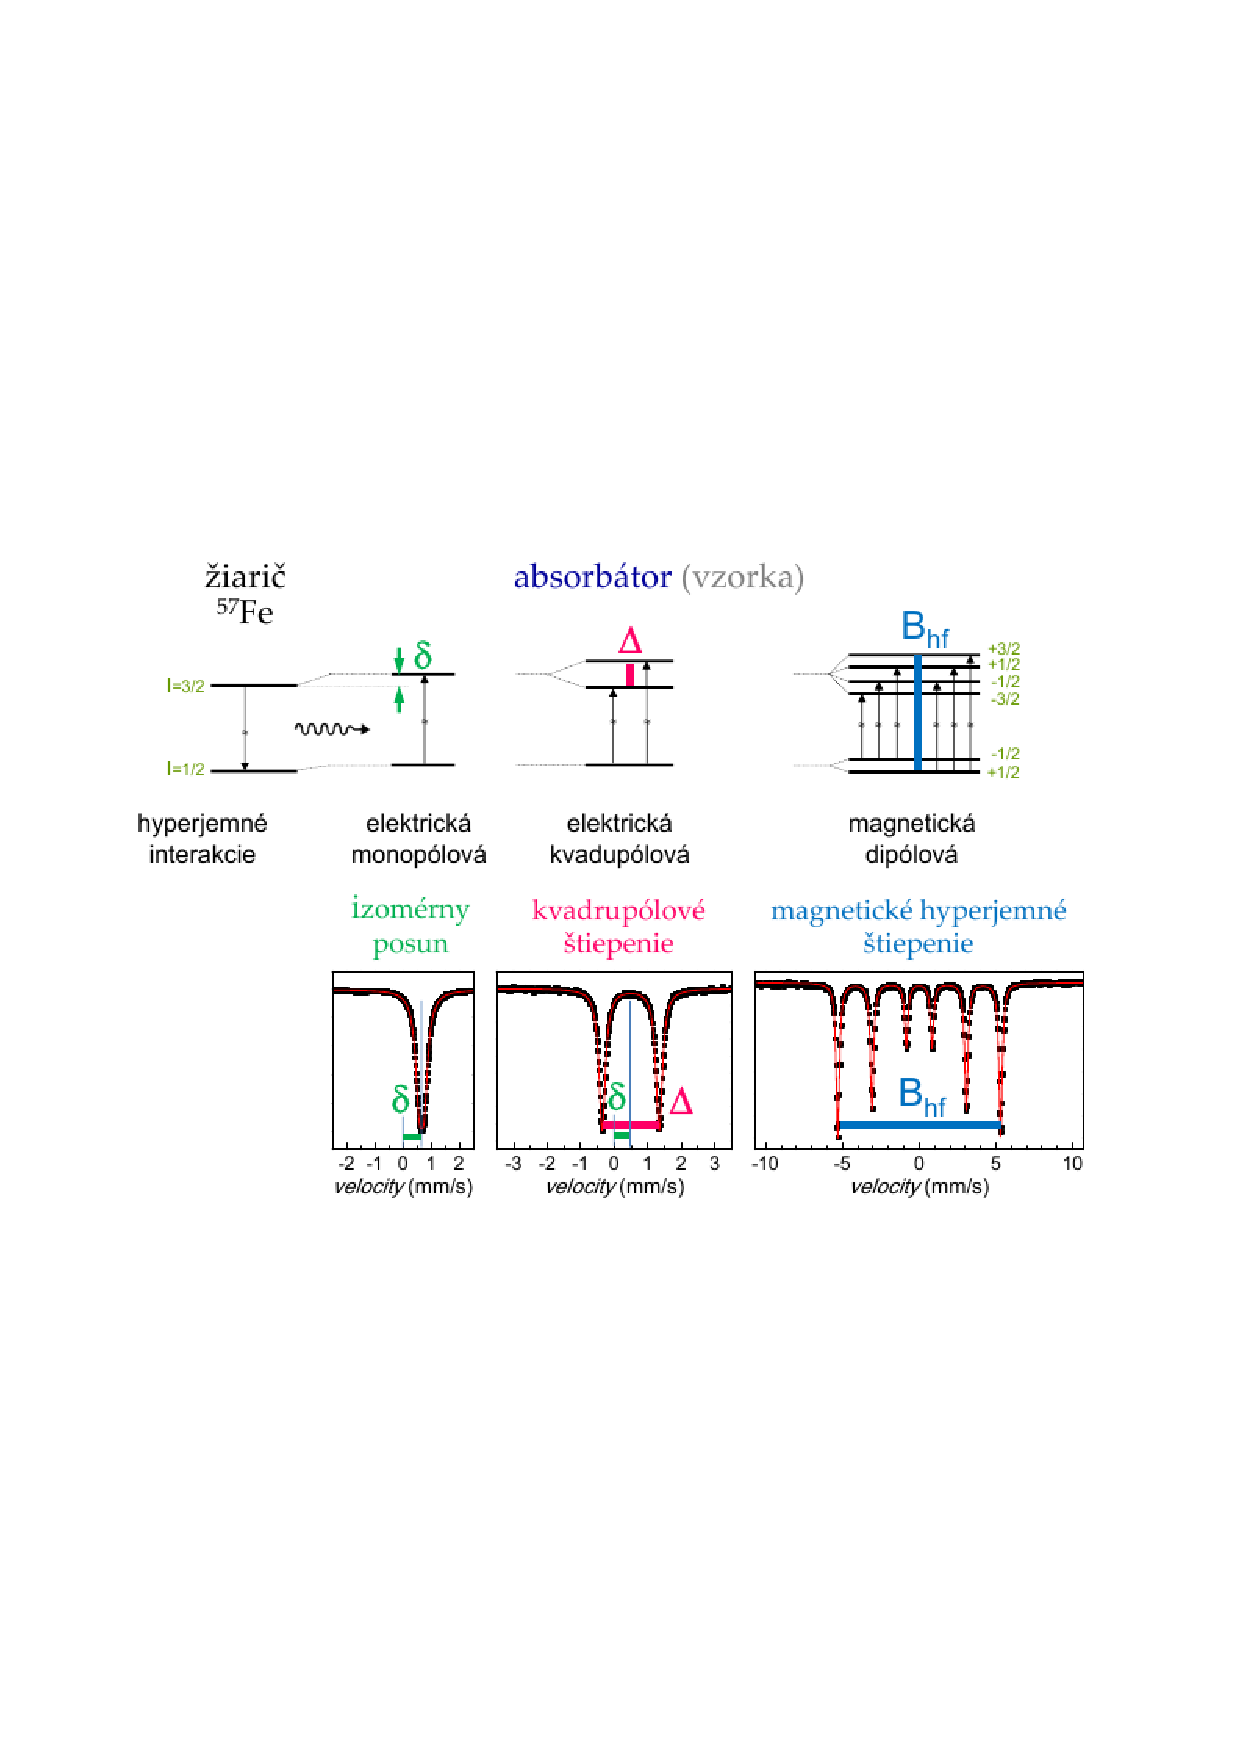
\includegraphics[width=0.8\linewidth, trim={2cm 10cm 2cm 10cm}, clip]{img/mossbauer_interactions.pdf}
   \caption{Hyperjemné interakce}
   \label{fig:6_2_mossbauer_hyperjemne_interakce}
\end{figure}

\textbf{Elektrická monopólová interakce:}

\begin{itemize}
\item interakce rozložení náboje jádra s hustotou elektronů v prostoru jádra 
\item izomerní posun $\delta = \dfrac{2\pi}{5} Ze^2 [R_e^2 - R_g^2] \cdot {\rho_a - \rho_s}$
\item pro excitovaný, resp. základní stav platí, že poloměr jádra se mění, stejně jako hustota
\item určuji s ohledem na referenční materiál (bcc-Fe)
\item udává informacee o charakteru vazeb, spinu, oxidačním čísle, elektronegativitě
\end{itemize}

\textbf{Elektrická kvadrupólová interakce:}

\begin{itemize}
\item interakce mezi jádrovým kvadrupólovým momentem a nehomogenitami elktrického pole
\item kvadrupólové štěpení: $\Delta = \dfrac{1}{2} eV_{zz} (1+\dfrac{1}{3}\eta^2)^{1/2}$ 
\item jaderná podmínka: elektrický kvadrupólový moment -- $eQ \neq$ 0 ($I$ > 1/2)
\item elektronová podmínka: gradient elektrického pole od elektronů $\neq$ 0 (příspěvek od mřížky a valenčních elektronů)
\item dává informaci o lókální symetrii, oxidačním stavu, charaktere vazeb, spinovém stavu

\end{itemize}
\begin{figure}[H]
   \centering
   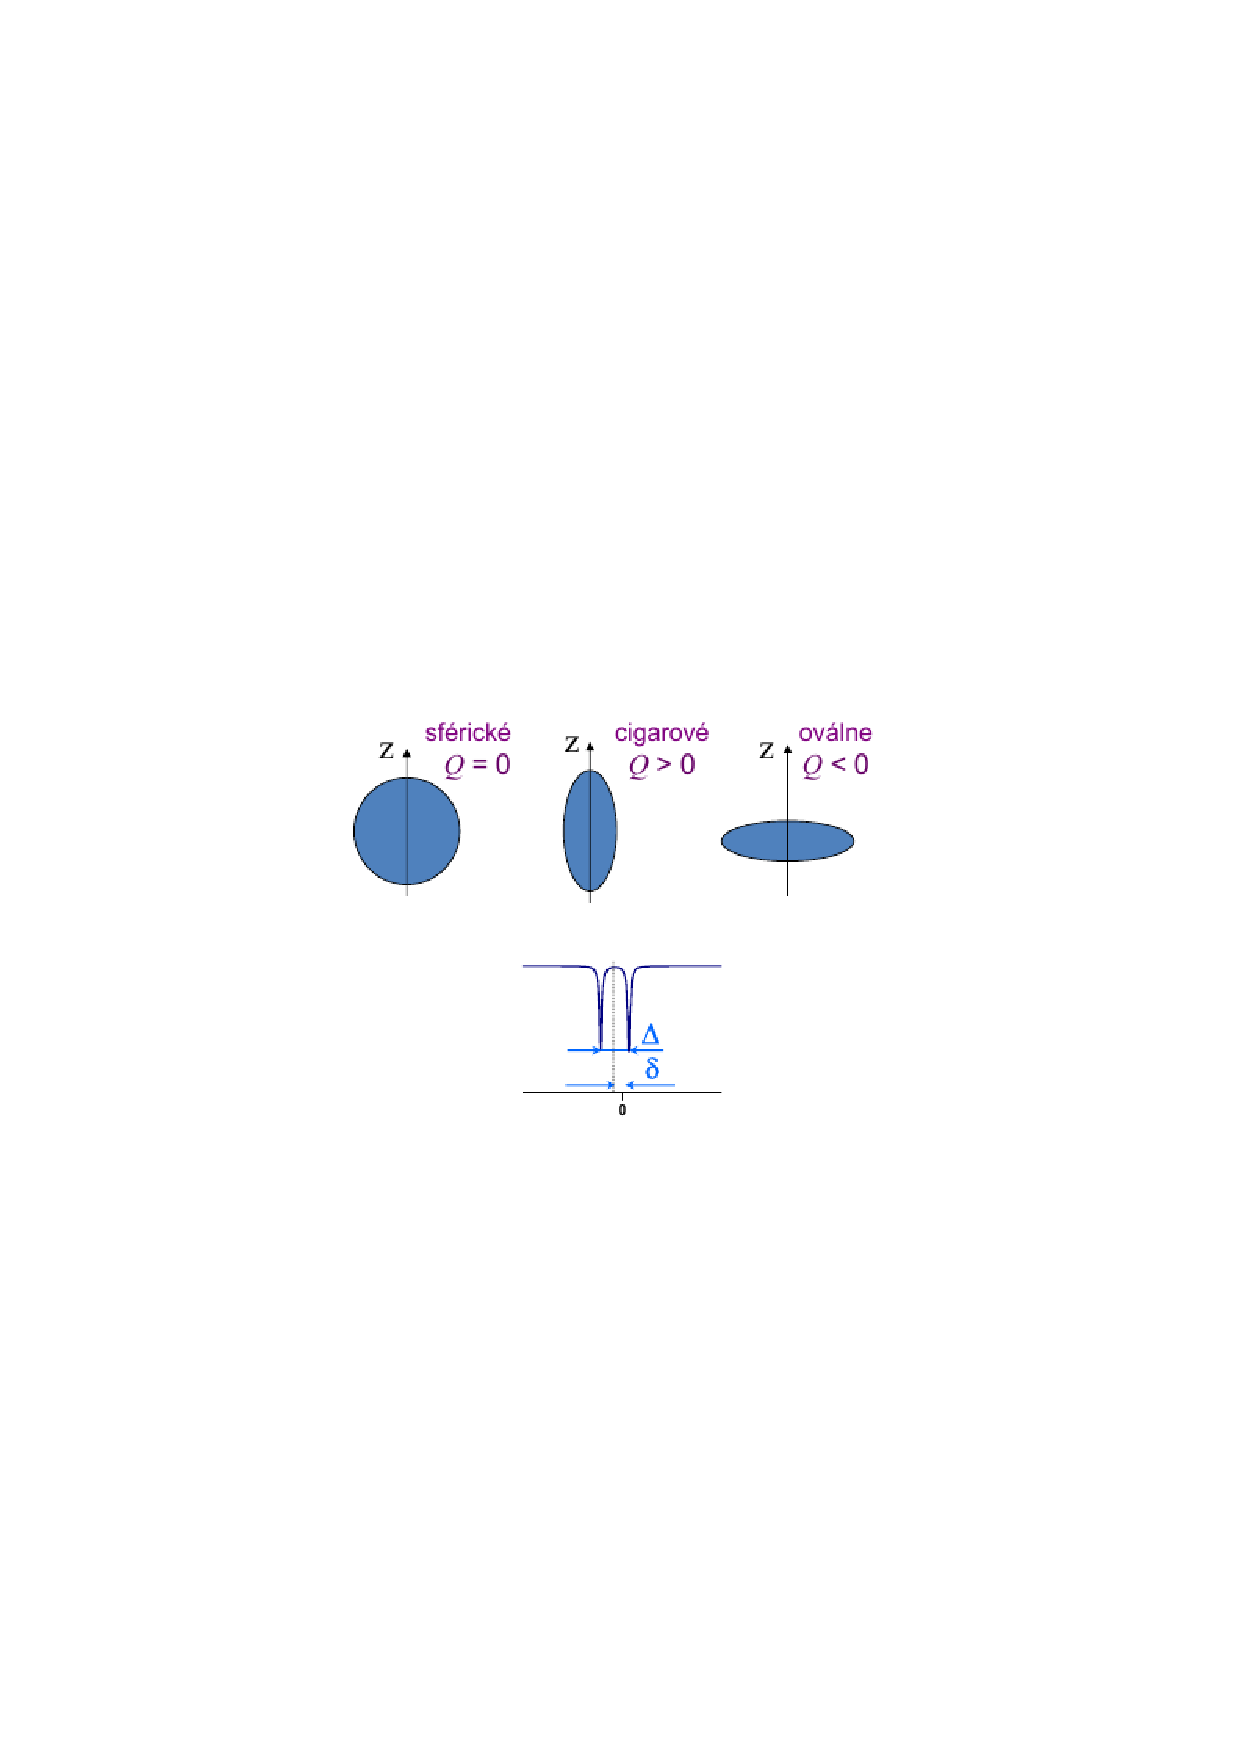
\includegraphics[width=0.5\linewidth, trim={4cm 11cm 4cm 11cm}, clip]{img/mossbauer_quadrupole.pdf}
   \caption{Elektrické kvadrupólové štěpení}
   \label{fig:6_2_mossbauer_electric_quadrupole}
\end{figure}

\textbf{Magnetická dipólová interakce:}

\begin{itemize}
   \item interakce magnetického momentu jádra s vnitřním nebo aplikovaným magnetickým polem
   \item $E_{m_1} = - \dfrac{\mu H m_1}{I} = - g_N \beta_N H m_1$
   \item magnetické štěpení hladin jádra (Zeemanův jev)
   \item jádrová podmínka: magnetický dipólový moment $\mu \neq 0$ (I > 0)
   \item elektronová podmínka: intenzita magnetického pole $H \neq 0$
   \item platí výběrová pravidla pro jádrový spin a magnetické kvantové číslo
\end{itemize}

\begin{figure}[H]
   \centering
   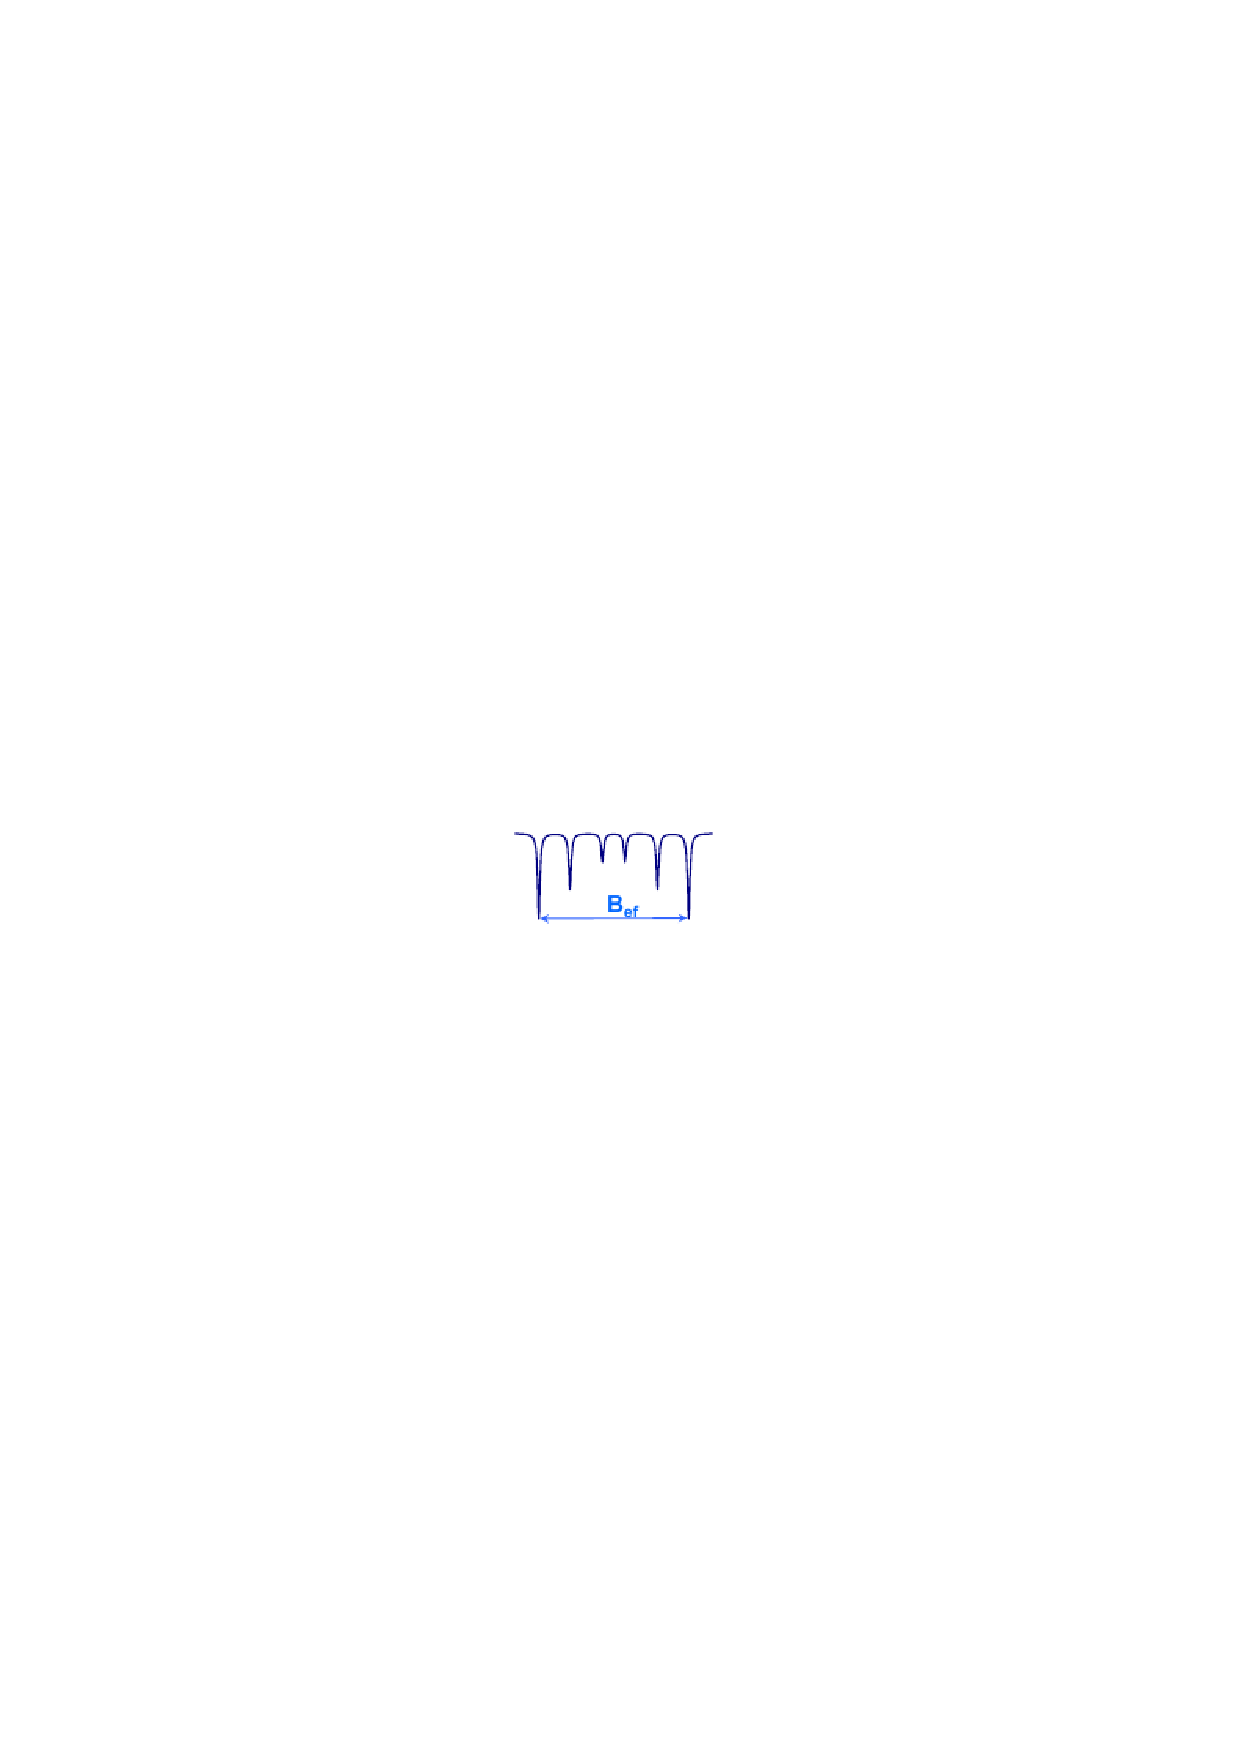
\includegraphics[width=0.5\linewidth, trim={5cm 14cm 5cm 14cm}, clip]{img/mossbauer_magnetic_quadrupole.pdf}
   \caption{Magnetické kvadrupólové štěpení}
   \label{fig:6_2_mossbauer_magnetic_quadrupole}
\end{figure}

\subsubsection{Kalibrace}

\begin{itemize}
   \item zdroj záření: $^{57}$Co v matrici Rh, Pd, Cu, Cr
   \item kalibrací ryhlostní stupnice (převedu rychlost na energii)
   \item kalibrační absorbátory - bcc-Fe, $\alpha$-Fe$_2$O$_3$
   \item nastvaení nulové rychlosti
\end{itemize}

\subsubsection{APlikace Mossbauerovy spektrometrie}

\begin{itemize}
   \item strukturní informace, stechiometrie, substituce, nekrystalické systém
   \item identifikace fází
   \item Fe2+ a Fe3+
   \item energetické rozlišení 1 : 10$^{13}$
   \item teplotní a tlakové studie
\end{itemize}

\begin{figure}[H]
   \centering
   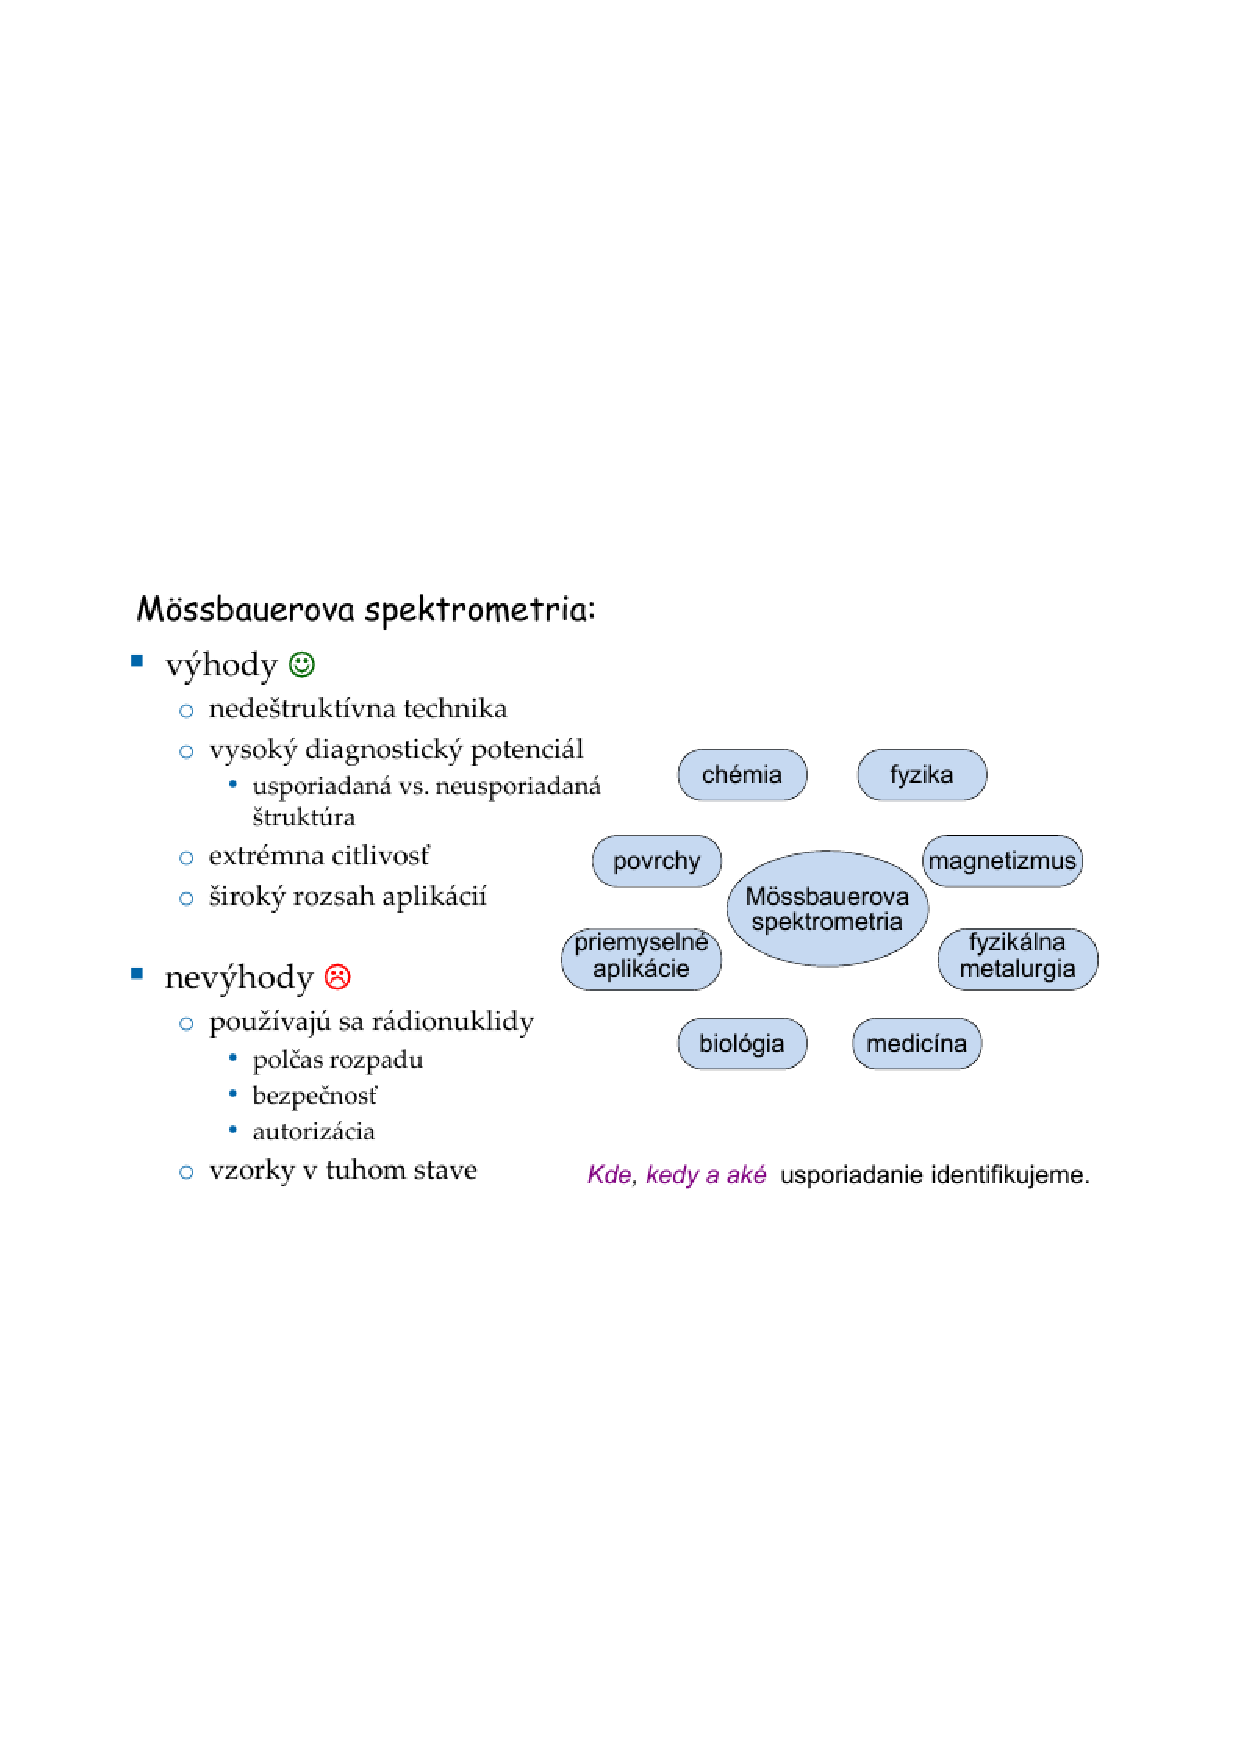
\includegraphics[width=0.5\linewidth, trim={2cm 10cm 2cm 10cm}, clip]{img/mossbauer_shrnuti.pdf}
\end{figure}

\subsection{Elektron-pozitronová anihilační spektroskopie}

Udává unikátní informace o defektech v pevných látkách (především vakance, dislokace, shluky vakancí, hranice zrn - principiálně se jedná o oblast se sníženou hustotou kladného náboje -- od jader :D $\rightarrow$ potenciálov jáma pro záchyt pozitronů).

Zdroje pozitronů:

\begin{itemize}
	\item beta+ radionuklidy: jádra bohatá na protony (p $\rightarrow$ n + $\beta$ + + $\nu$), Na-22, Cu-64, Co-58
	\item Produkce e--e+ párů z vysokoenergetických fotonů gama: impuzní zdroj e+
	\item Jaderné reakce: Cd-113(n, gama)Cd-114, Cu-63(n, gama)Cu-64, kontinuální zdroj s vysokou intenzitou
\end{itemize}

$\rightarrow$ Zdroje pro PET: C-11, N-13, O-15, \textbf{F-18}, Ga-68 - výroba: nejčastěji cyklotron

Princip anihilace: pozitronový zářič $\rightarrow$ interakce pozitronu s elektronem $\rightarrow$ vznik dvou fotonů o energii 511 keV (nejpravděpodobnější proce).

\begin{itemize}
    \item anihilace nenastává okamžitě - mezitím: vázaný stav - pozitronium (para a orto pozitronium - podle toho jestli stejný nebo opačný spin pozitronu a elektronu a také podle toho jinak dlouho trvají)
\end{itemize}

\subsubsection{Experimentální techniky}

\begin{itemize}
    \item Doba života pozitronů -- vyzářen pozitron a gama $\rightarrow$ měří se vyzáření pozitornu a gama
    \item Dopplerovo rozšíření -- koincidenční změření energie obou anihilačních fotonů $\rightarrow$ charakterizace chemického okolí defektů
    \item Úhlové korelace
\end{itemize}

\begin{figure}[H]
    \centering
    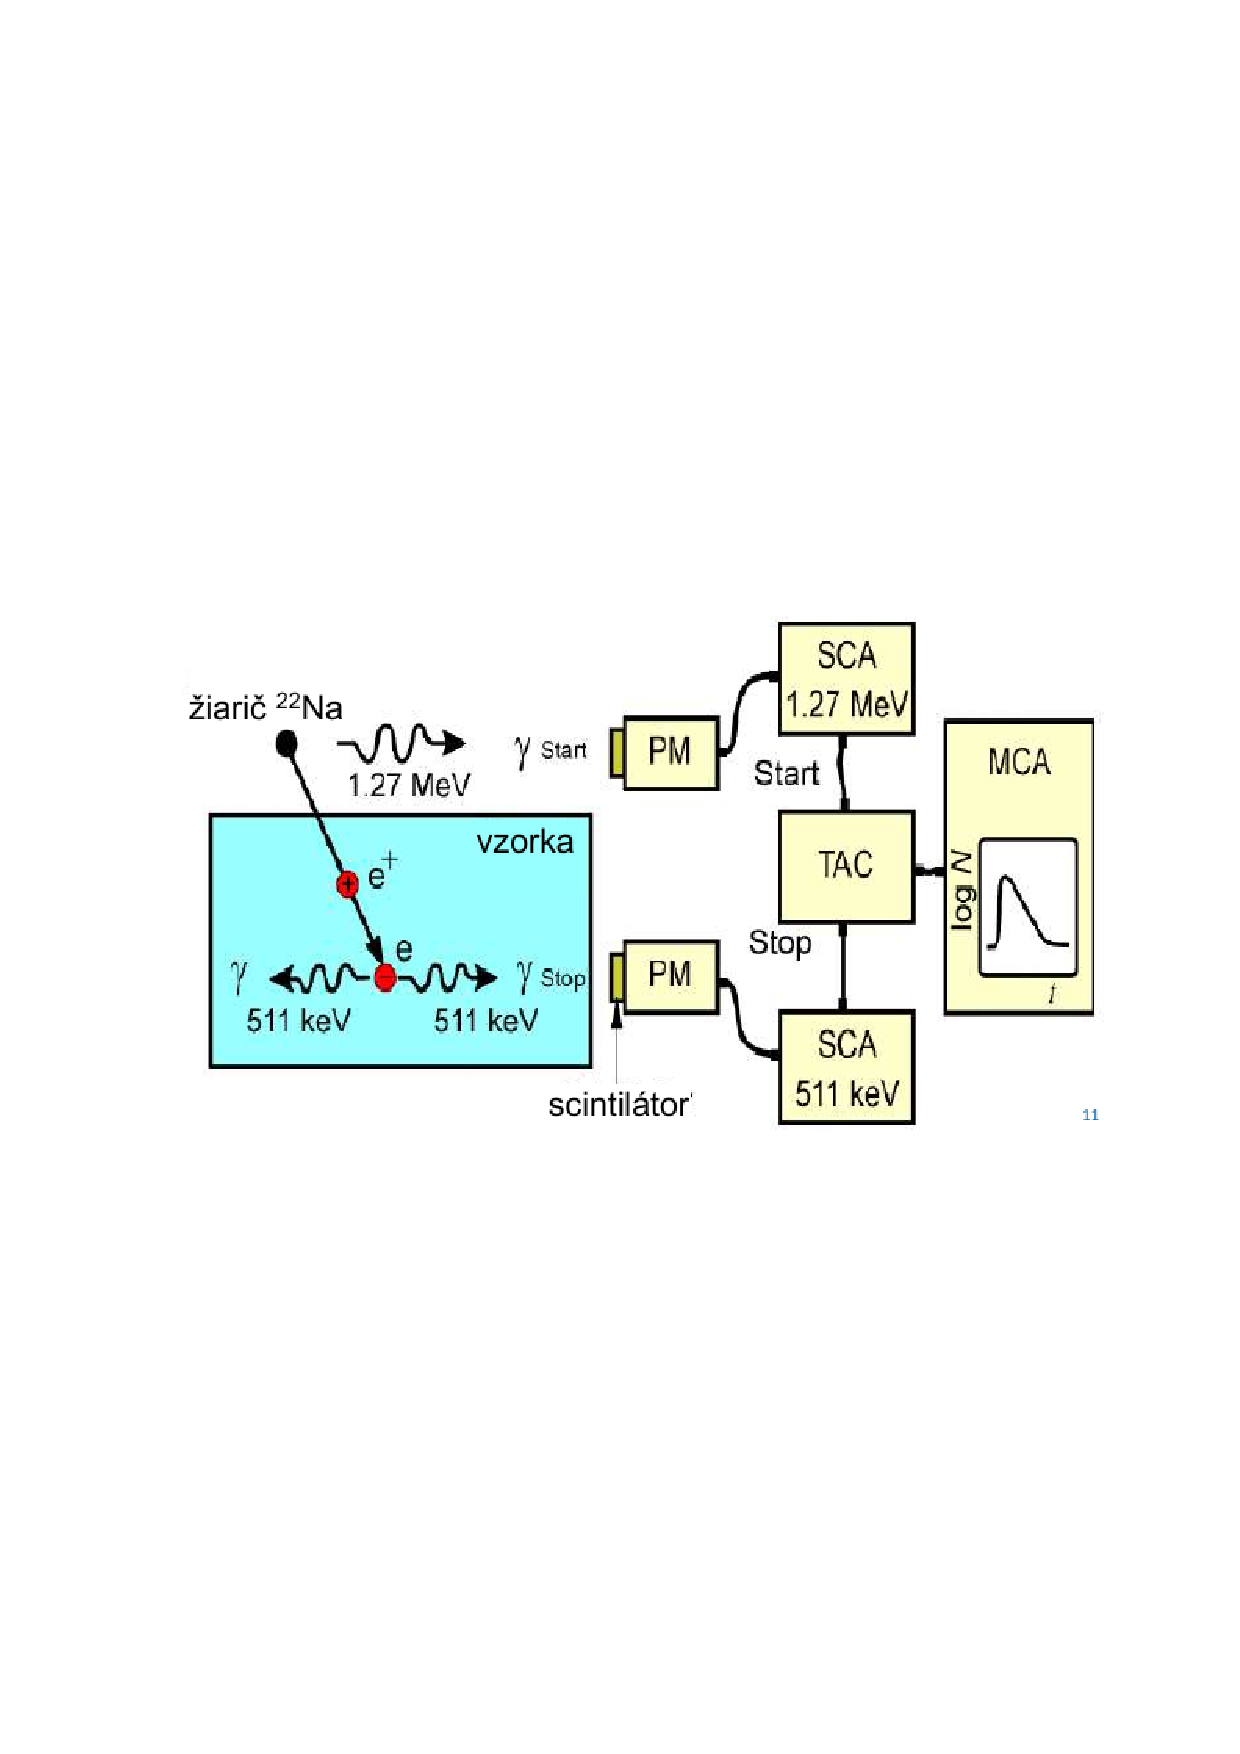
\includegraphics[width=0.8\linewidth, trim={2cm 10cm 2cm 10cm}, clip]{img/pas_doba_zivota.pdf}
    \caption{Metoda doby života pozitronů.}
    \label{fig:6_2_pas_doba_zivota}
\end{figure}

\begin{figure}[H]
    \centering
    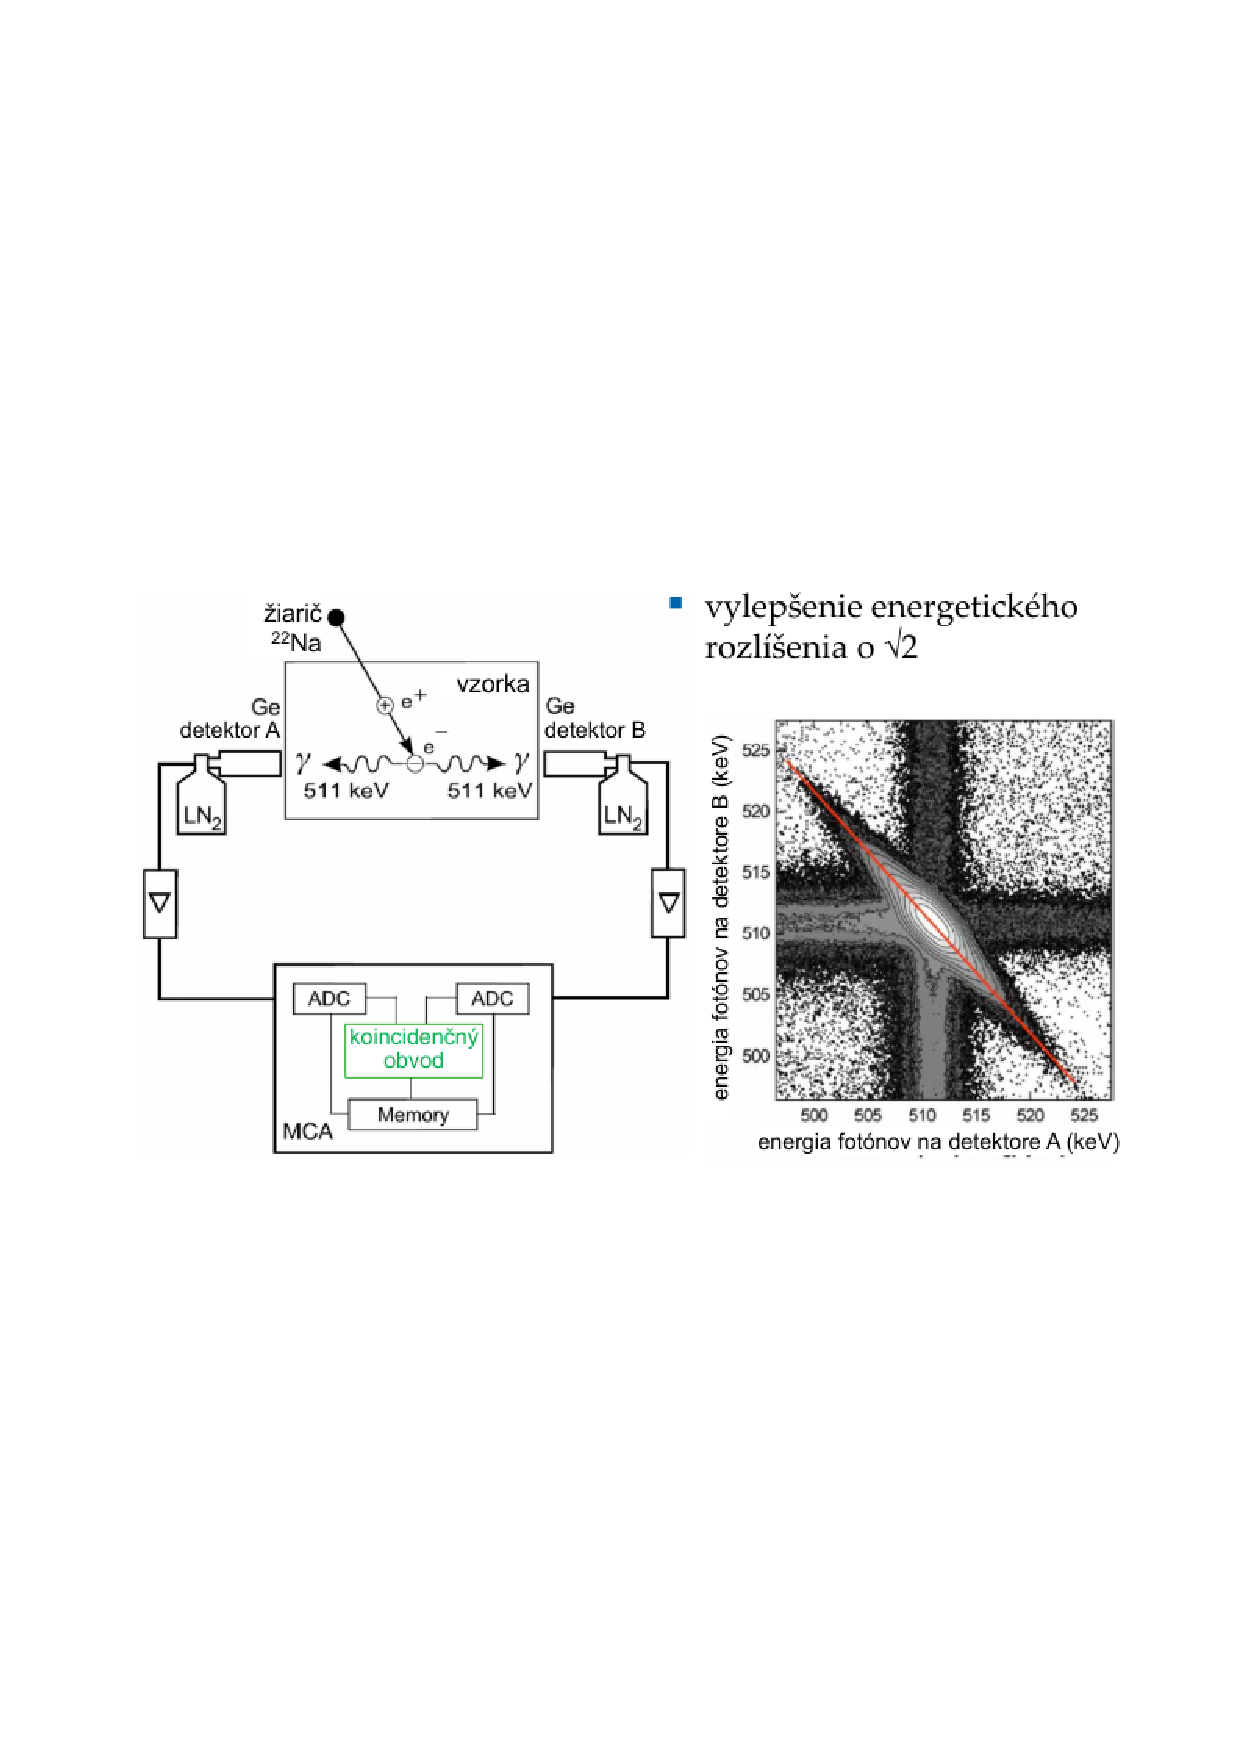
\includegraphics[width=0.8\linewidth, trim={2cm 10cm 2cm 10cm}, clip]{img/dopplerovo_koincidencni_zapojeni.pdf}
    \caption{Metoda Dopplerova rozšíření- koincidenční zapojení}
    \label{fig:6_2_pas_dopplerovo_rozsireni}
\end{figure}

\subsection{Neutronová aktivační analýza}

\begin{itemize}
    \item Je založena na aktivaci chemických prvků přítomných v analyzovaném vzorku. 
    \item Jedná se o jednu z nejvíce citlivých metod chemické analýzy
    \item Obvykle je aplikována s využitím měření následného rozpadu aktivovaných prvků (měření gama)
    \item Existuje i metoda s měřením okamžitého záření a ta je využívána pokud produkt reakce má velmi krátký poločas rozpadu a nebo vzniká stabilní produkt.
    \item Pro NAA se dají vyuźít neutrony všech energií, avšak nejčastěji se využívají tepelné, a to kvůli větší dostupnosti neutronů při této energii a také kvůli energetické závislosti účinných průřezů, které mají v této oblasti vysoké hodnoty.
    \item Množství aktivovaných RA atomů daného prvků ve vzorku je přímo úměrné množství těchto atomů a proto se dá využít i pro kvantitativní analýzu.
    \item Indukovaná aktivita závisí na době ozařování a poločasu rozpadu, přičemž okolo $10x T_{1/2}$ dosahuje akivita saturované hodnoty.
    \item Po aktivaci jader v analyzovaném vzorku následuje měření radioaktivity vzorku a identifikace RN na základě energie a intenzity emitovaného gama záření a s ohledem na poločas rozpadu.
    \item Množství studovaného prvku lze získat z naměřené aktivity s tím, že je nutno brát v potaz:
    \begin{itemize}
        \item Hustotu toku neutronů (resp. energetické spektrum)
        \item Energetickou závislost účinných průřezů
        \item Dobu ozařování
        \item Poločas rozpadu
        \item Detekční účinnost trasy (geometrie, stínění, mrtvá doba atd.)
        \item Dobu měření
        \item Dobu chladnutí (přesun po ozařování k detektoru)
    \end{itemize}
\end{itemize}
 
\textbf{Rozdělení NAA}
\begin{itemize}
    \item Absolutní
        \begin{itemize}
            \item Z přímého měření aktivity umožňuje stanovit množství zkoumaného izotopu, avšak vyžaduje k tomu přesnou znalost neutronového spektra, účinných průřezů s ohledem na energetický rozsah neutronového pole.
            \item Málo kdy využívaný přístup protože přesná znalost neutronového spektra není v praxi obvykle k dispozici
        \end{itemize}
    \item Porovnávací:
        \begin{itemize}
            \item Srovnávání aktivity RN ve zkoumaném vzorku s jeho aktivitou v podobě standardu/etalonu o známé hmotnosti a složení, který byl ozářen za stejných podmínek jako zkoumaný vzorek
            \item Při srovnávací metodě se nevyužívají hodnoty účinných průřezů ani neutronový tok a v případě stejné geometrie při detekci/měření tak ani absolutní detekční účinnost (pro oba měřené je to stejné, tak to není vyžadováno)
            \item Vysoká přesnost, avšak časově náročné pokud vzorek obsahuje vícero prvků, protože pro každý je nutné mít etalon zvlášť.
        \end{itemize}
    \item $k_0$ metoda
        \begin{itemize}
            \item využívá $k_0$ faktory, které se stanovují na základě jaderných dat v kombinaci s experimentálním stanovením.
            \item nezávisí na neutronovém toku a charakteristikách detektoru
        \end{itemize}
    \item Instrumentální NAA -- toto známe a děláme na KJR.
        \begin{itemize}
            \item Nedestruktivní metoda pro stanovení vícero prvků v rámci jednoho měření
            \item Nežádoucím efektem je vzájemné ovlivňování prvků = Vznik jednoho RN reakcemi na dvou různých prvcích (26Mg(n;$\gamma$)27Mg a 27Al(n;p)27Mg) = Tento problém je ovšem řešitelný v případě, kdy jeden z prvků produkuje i další radioaktivní nuklidy a dále také pokud je rozdíl v energetické závislosti účinných průřezů na energii neutronů, tak se dá použít vhodný filtr jako např Cd.
            \item V praxi se měří tak, že se vzorek ozáří v reaktoru na saturovanou hodnotu, pak se nechá vychladnout (snížení aktivity) pokud je moc naaktivovaný a pak se odnese do gama spektrometru a měří se gama záření z rozpadu RN. Z naměřeného spektra se poté stanovuje kvantita a kvalita složení materiálu.
        \end{itemize}
\end{itemize}

\subsubsection{Nastavení experimentálních parametrů}
\begin{itemize}

            \item V rámci tohoto měření, tak je vhodné mít odladěnou dobu ozařování (ať to není zbytečně moc a aktivita dlouhodobě žijících RN není moc vysoká)
            \item dobu vymření (chceme minimalizovat aktivitu všech RN kromě toho, který chceme měřit)
            \item Doba měření (měla by být kratší než nějaký významnější pokles aktivity vzorku - pak mi do toho začne hrát roli pozadí a Rn, K a U)
            \item při ozařování dochází ke vzniku vícero aktivačních produktů z jednoho prvku (pro ověření lze měřit dlouho a zaměřit se na ověření přes poločas rozpadu). Popřípadě aktivační produkty obvykkle emitují $\gamma$ fotony o vícero energiích, čímž je možné taky jednoznačně stanovit.
            \item Měřící geometrie (mrtvá doba)
            \item Velikost vzorku: zbytečně velký vzorek představuje riziko samostínění, samoabsorpce gama záření či zbytečně velkou aktivitu nebo problematické manipulace (to platí i pro zbytečně malý vzorek).
            \item Tok primárních částic přímo ovlivňuje úroveň produkované aktivity.
            \item Ve výsledném výpočtu reakční rychlosti, resp. obecně měření je nutné zohlednit několik faktorů = plocha pod píkem při měření, počet částic v látce na počátku, oprava na čistou dobu měření, doba ozařování, rozpad při vymírání, rozpad při měření, Radiační výtěžek (oprava na intenzitu gama přechodu), oprava na efektivitu detektoru pro danou geometrii (detekční účinnost). Korekce na nerovnoměrné ozařování, korekce na samoabsorpci.
        \end{itemize}

\textbf{Využití a aplikace NAA:}
\begin{itemize}
    \item Monitoring životního prostředí
    \item Zajištění jakosti v průmyslu
    \item Hygienické studie
    \item Certifikace referenčních materiálů
    \item Stopové prvky
    \item Kvalita půdy
    \item Analýza uhlí
\end{itemize}